\documentclass[a4paper,11pt, DIV=12]{scrartcl}
\usepackage[utf8]{inputenc}

\usepackage{graphics}
\usepackage{epsfig}
\usepackage{amsmath}
\usepackage{amssymb}
\usepackage{amsfonts}
\usepackage{booktabs}
\usepackage{biblatex}
\usepackage{hyperref}
\usepackage{caption}
\usepackage{subcaption}
\usepackage{array}
\usepackage{adjustbox}
\usepackage{tabularx}
\usepackage{wrapfig}
\usepackage{svg}
\usepackage{xcolor}

\definecolor{negative}{HTML}{f1cc40}
\definecolor{positive}{HTML}{6f91d9}
\definecolor{query}{HTML}{141a58}

\graphicspath{ {./img/} }
\allowdisplaybreaks
\addbibresource{sources.bib}

\newlength{\tablesize}

\newcommand{\x}{\boldsymbol{x}}
\newcommand{\y}{\boldsymbol{y}}
\newcommand{\vp}{\boldsymbol{v}^+}
\newcommand{\vm}{\boldsymbol{v}^-}
\newcommand{\ve}{\boldsymbol{v}}

\title{Examination of Unpaired Translation Methods for Near-Infrared Image Colorization}
\author{Ayk Borstelmann\footnote{student ID number: 3441004, address: Koenigswinterer Str. 204, 53227 Bonn}}

\begin{document}

\maketitle

\section{Introduction}
For wildlife monitoring, typically camera traps are used. During daylight, normal cameras succeed in capturing detailed images.
But in the absence of daylight \textit{near-infrared} (NIR) cameras or normal cameras using incandescent lighting are necessary.
NIR cameras offer a significant advantage over conventional cameras using incandescent lighting.
Light flashes are visible to animals and may frighten them, which leads animals to avoid the camera location afterward.
Near-infrared light, however, is for most animals not visible, thus cannot scare them.
However, unlike colored RGB images, NIR images lack colorization, which is essential for human comprehension and interpretation of visual information.
Also, some classification- and animal detection solutions may benefit from three-channel RGB images.
Therefore, the conversion of NIR images to colored RGB images can combine the advantages of both methods:
Detail-rich images without scaring animals, that humans can easily interpret and classification and animal detection systems can benefit from.

Although colorizing NIR images is closely related to colorizing grayscale images (\textit{image colorization}), it differs in one important property:
The luminance of grayscale images is the same as the luminance of colored images, thus only chrominance must be estimated by image colorization systems.
The objects' reflection properties of near-infrared light differ from those of light from the visual spectrum.
Consequently, due to the differing luminance between RGB and NIR images, conventional image colorization techniques cannot be applied.

Supervised solutions for this problem exist, but require NIR, RGB image pairs with pixel-to-pixel registration, and temporal synchronization:
For each given NIR image the corresponding RGB image must have the same information on the pixel locations on both images and both images must be captured simultaneously to account for motion.
However, there are many datasets consisting only of NIR images from the night and RGB images from the day.
This results in an unpaired image translation problem for which unsupervised learning techniques must be applied.

\textit{Generative Adversarial Networks} (GANs) are a common approach for unpaired image translation.
Two of such GAN architectures, \textit{CycleGAN} \cite{mehri2019colorizing} and \textit{CUT} \cite{cut} are compared in the context of wildlife NIR image colorization.
Because CUT has shown superior performance over the original CycleGAN for many image translation tasks \cite{cut}, we apply and analyze it in this context.
However, our results show that CUT does not surpass a NIR colorization-tuned version of CycleGAN \cite{mehri2019colorizing}.
Also, it is shown that for the general image colorization problem (grayscale $\rightarrow$ color), this observation also remains.
Both methods are evaluated with respect to the mentioned benefits of colorizing NIR images.
Furthermore, requirements for the training datasets are found that significantly affect the learning success.

\section{Related Work}
NIR colorization has many applications in addition to wildlife monitoring, for example in driver assistance systems or surveillance cameras.
As a result, the research area of computer vision has studied image colorization during the last decades, therefore many solutions exist.
Recently, deep learning-based approaches, especially convolutional neural networks (CNNs), have shown great success in colorizing NIR images \cite{limmer2016infrared}.
Additionally, the recent developments of U-Net \cite{unet} and ResNet \cite{resnet}, which incorporate skip connection to significantly improve the network's performance, have also affected
the NIR colorization solutions. As a result, these networks are now widely used \cite{cyclegan_orig,mehri2019colorizing,cut,dong2018infrared}.

In the case of NIR colorization, the solutions are divided into paired and unpaired image translation problems and thus supervised and unsupervised learning techniques are applied respectively.
For paired image translation, pixel-to-pixel registration and temporal synchronization are required for each image pair, which adds additional challenges.

Limmer \textit{et al.} used a dataset acquired by a specialized multi-CCD camera which ensures the image pair requirements \cite{limmer2016infrared}.
Additionally, Limmer \textit{et al.} proposed to use Deep Multiscale CNNs.
In pre-processing, a normalized image pyramid is constructed by the NIR input and in post-processing, the CNN output is enriched with details from the input image \cite{limmer2016infrared}.
In later work, Dong \textit{et al.} introduced an S-Shape network consisting of one U-Net-based encoder "ColorNet" and a shallow network that generates an edge loss function "EdgeNet" \cite{dong2018infrared}.
Dong \textit{et al.} achieved pixel-to-pixel registration using geometric transformations and feature-based correspondence methods \cite{dong2018infrared}.

In recent years, GAN-based methods have emerged as a powerful approach to unpaired image translation, which can be used for NIR image colorization without the need for paired training data.
This is especially useful if such data cannot be obtained, for example, due to dataset limitations.
GANs by default tend to lose the content of the input image. CycleGAN as an architecture proposed by Zhu \textit{et al.} uses a cycle consistency loss between the input and the generated image to solve that problem \cite{cyclegan_orig}.
It utilizes ResNet \cite{resnet} as generator networks \cite{cyclegan_orig}.
Gao \textit{et al.} trained CycleGAN on a wild-life dataset and show improved recognition results on the generated images compared to the NIR images \cite{cyclegan_camera_traps}.

Mehri \textit{et al.} proposed a version of CycleGAN, specifically designed for the task of colorizing NIR images, which incorporates enhanced loss functions and utilizes U-Net as a generator \cite{mehri2019colorizing}.
In a later work, Park \textit{et al.} proposed \textit{contrastive unpaired translation} (CUT) for unpaired image translation \cite{cut}.
It outperforms the original CUT in many tasks \cite{cut}, thus we investigate it in the context of wild-life NIR colorization.
We compare those two GAN-based methods and concentrate on the unpaired image translation problem.

\section{Dataset}
While examining both proposed methods for their suitability for near-infrared colorization, multiple datasets
and two data sources \textit{Caltech Camera Traps} \cite{caltech} and \textit{Snapshot Serengeti} \cite{serengeti} were used.

\subsection{Caltech Camera Traps}
\textit{Caltech Camera Traps} (CCT) is a dataset consisting of $243.100$ images from $140$ camera locations
in the southwestern United States with $21$ animal label categories \cite{caltech}.
In particular, it primarily contains near-infrared images for the night and regular RGB images for images captured during the day.
Approximately $70 \%$ of the overall image set is labeled empty.
Annotations are provided in the \textit{COCO Camera Traps} format, describing meta information via JSON \cite{caltech}
This allows an automatic parsing of the available images as well as efficient access to information about
the images, which comes in useful when creating sub-datasets for training networks.

\subsection{Snapshot Serengeti}
In contrast to the CCT dataset, \textit{Snapshot Serengeti} is a much larger dataset and comes from the Snapshot Serengeti National Park in Tanzania.
It consists of $7.1$ million images through seven seasons of the Snapshot Serengeti Project \cite{serengeti}.
There are $61$ labeled species, where approximately $76\%$ of the images are labeled empty.
Similar to the CCT dataset, Snapshot Serengeti contains near-infrared images as well as RGB images and
is annotated in the COCO Camera Traps format \cite{serengeti}. Therefore, dataset tooling can be used for both datasets.
Unlike the CCT dataset, Snapshot Serengeti employed multiple cameras for images captured at night.
Scoutgard's SG565 cameras produce RGB \textbf{night} images using an \textit{incandescent} flash and DLC Covert II cameras use an infrared flash and therefore produce NIR night images \cite{serengeti}.

\subsection{Subset Generation}
Since both datasets (CCT and Snapshot Serengeti) are substantially larger than processable for training, choosing a subset of these images is essential.
The requirements for this subset strongly influence the training performance of the translation models.

\begin{enumerate}
   \item Both network architectures require the dataset to be divided into an input domain (NIR) and an output domain (RGB). \label{item:requirement-split}
   \item To gain model performance in the main objective, which is to colorize the NIR images of \textit{animals}, it is important to choose only images that contain animals. \label{item:requirement-animal-filter}
   \item Training with a variety of image locations proves to decrease overfitting for the translation, and therefore a uniform distribution of the available locations should be approximated.
         Additionally, utilizing a random crop for each image can also help mitigate overfitting, and therefore, it is suggested. \label{item:requirement-weighted-sampling}
   \item Since most NIR images are taken at night, the network should not be influenced to solve the more difficult
         task of translating images from NIR night to RGB day. This can be achieved by only allowing night images for both
         domains. \label{item:requirement-night}
\end{enumerate}


The \ref{item:requirement-animal-filter}., \ref{item:requirement-weighted-sampling}. and \ref{item:requirement-night}. requirements are all achievable by using the information provided in the COCO format, and therefore,
are already obtainable before downloading a single image.
Only choosing images with animals (\ref{item:requirement-animal-filter}.) is done by a simple filter on the data source before sampling.
The approximately uniform distribution of locations (\ref{item:requirement-weighted-sampling}.) can be archived using a weighted sampling with the inverse of location occurrences as weight.
Filtering for only night images (\ref{item:requirement-night}.) can also be achieved only using metadata:
The COCO format documents the time of recording. Using time zones and geolocations, individual time frames for each day of the year can serve as filters for night images.

Since the COCO format does not provide information about which item is a NIR- and which item is an RGB image (\ref{item:requirement-split}.) \cite{caltech}, that information is not available before downloading.
Because both data sources provide their NIR images with \textit{colored} logos, they are stored in an RGB image where the actual image section has equal values over all three channels.
Therefore, a pragmatic solution is to download the images and compare the three channels in a cropped version of the image (without the logo section).

This whole process can be automated in the form of a mix between a rejection- and an importance sampler:
It samples from the filtered data source with weights by location, downloads the image and rejects a sample if the desired amount of NIR- or RGB images is reached.
Finally, the produced subset can be stored in a compact format to achieve reproducibility across systems and reduce computational time.

\section{Proposed Methods}

For image translation, a mapping function $G: \mathcal{X} \to \mathcal{Y}$ shall be learned.
In our case, $\mathcal{X}$ is the input domain of the near-infrared images, whereas $\mathcal{Y}$ is the output domain of the colored RGB images.
For the training, two sets $X = \{\x \in \mathcal{X}\}$, $Y = \{\y \in \mathcal{Y}\}$ are given.
For the unpaired image translation, the mapping function must be learned without any existing $\x \in X$ for which $G(\x)=\y$ is known.
Therefore, supervised learning techniques are not applicable, and unsupervised learning methods must be considered.

\textit{Generative Adversarial Networks} (GANs) provide a way of learning this function by declaring the objective that, for a $\x \in \mathcal{X}$, $G(\x) = \hat{\y}$
should be indistinguishable from images from $\y \in \mathcal{Y}$. GANs achieve this by splitting the training architecture into two networks:
The \textit{generator} $G: \mathcal{X} \to \mathcal{Y}$ that learns the relationship between the two domains and the \textit{discriminator} $D: \mathcal{Y} \to \mathbb{R}$ that learns to
classify possible images from $\mathcal{Y}$ as "real" or "generated".
Both networks optimize each other and play a min-max game:
The generator tries to fool the discriminator into classifying the generated image as "real" and thereby learns to produce \textit{indistinguishable} images from $Y$.
Additionally, the discriminator tries to detect generated images, while also learning the features of the domain $\mathcal{Y}$ by classifying those as "real".

Although this method has already proven to perform well for image translation, it has issues preserving the content.
GANs in general are not restricted in training to map the actual \textbf{content} from the given image
$\x \in X$ to the image produced $G(\x) \in Y$.
For example, one could imagine that the mapping function which maps all $\x$ to some real $\y \in Y$ ($G(\x) = \y$) should perform exceptionally well in terms of its training loss, since the produced image should always be classified as "real".
This case is called \textit{mode collapse} and can be weakened by adding additional structure to the training.

In the following, we will concentrate on two options:
1. Using a \textit{cycle consistency loss} which was introduced by Zhu \textit{et al.} for the network \textit{CycleGAN} \cite{cyclegan_orig}
and 2. using a \textit{contrastive loss} that Park \textit{et al.} introduced into this environment for the network \textit{CUT} \cite{cut}.

\subsection{CycleGAN}
CycleGAN is a network architecture presented by Zhu \textit{et al.} and introduces a \textit{cycle consistency loss} for image translations using GANs.
The idea is that the translation between the two domains should be "cycle consistent", meaning that when translating an image from NIR to RGB and back
to NIR, both NIR images should be approximately equal.
Mathematically, this means that we have an additional function $F: \mathcal{Y} \to \mathcal{X}$ which is approximately the inverse of $G$. For a $\x \in \mathcal{X}$, $F(G(\x)) \approx \x$.
This is encouraged using a \textit{cycle consistency loss} \cite{cyclegan_orig}. We assume that if a $\x$ is recoverable from a $\y = G(\x)$ using $F$, the content of $\x$
is preserved in $\y$ \cite{cyclegan_orig} (\autoref{fig:cycle-gan}).

\begin{figure}[h]
   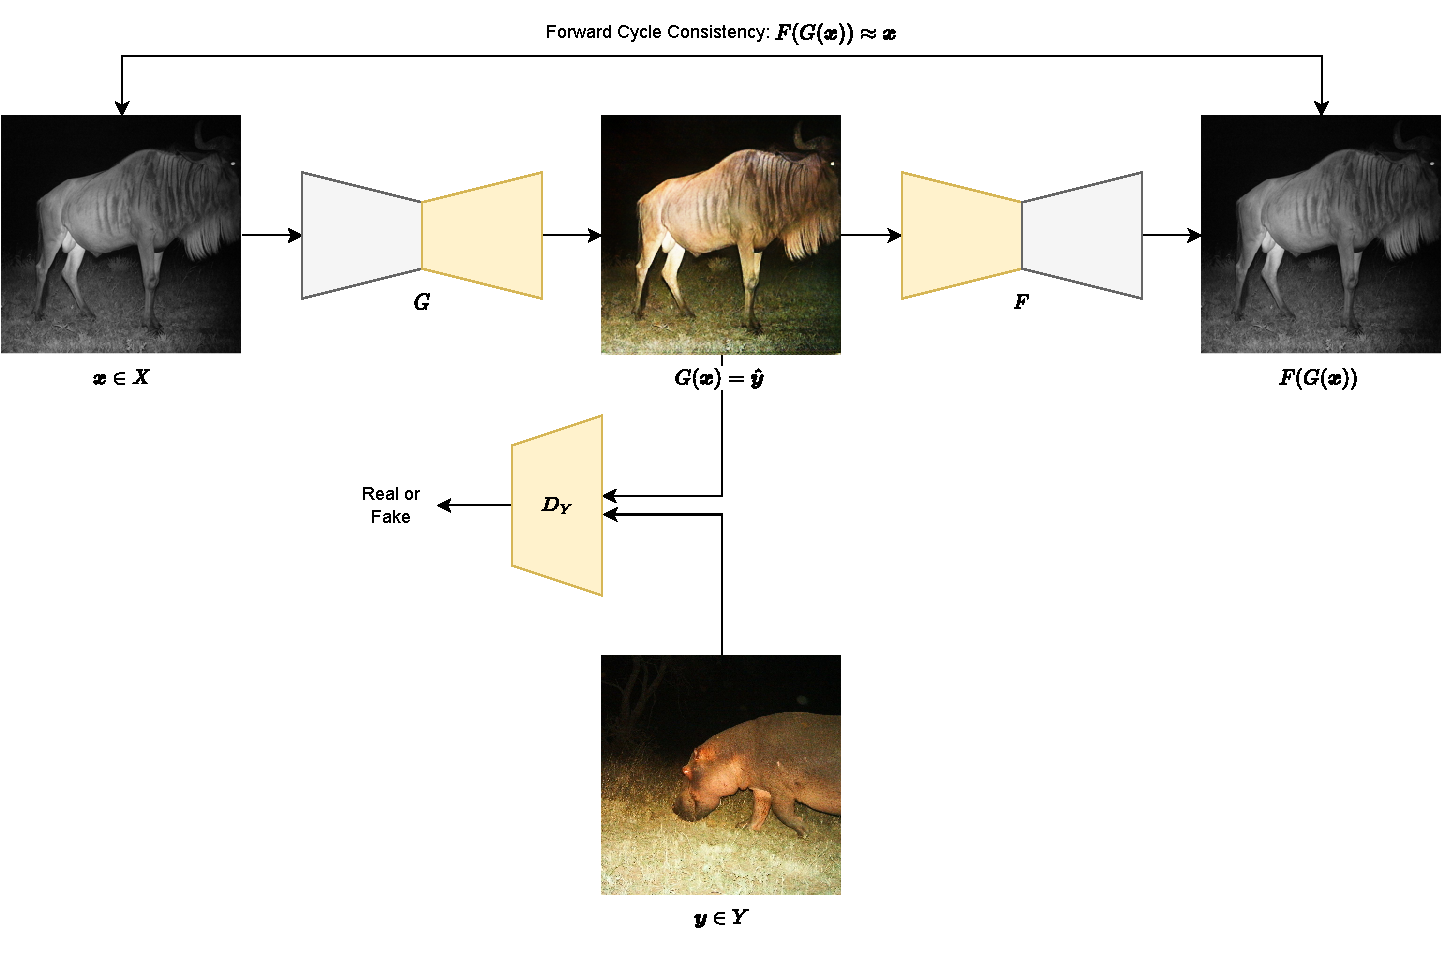
\includegraphics[width=\textwidth]{CycleGAN.pdf}
   \caption{
      \textbf{CycleGAN Schema.} Two generators $G$ and $F$ translate between both domains. Forward Cycle Consistency is ensured using the input and recovered NIR image.
      The discriminator $D_Y$ encourages the generator $G$ to learn the features of domain $\mathcal{Y}$ \cite{cyclegan_orig,mehri2019colorizing}.
   }
   \label{fig:cycle-gan}
\end{figure}

\subsubsection*{Cycle Consistency Loss}
This objective is written as a loss function $\mathcal{L}_{cyc}(G, F)$ which uses an L1 norm to encourage cycle consistency (\autoref{eqn:cyc}).
In addition to \textit{forward cycle consistency}, CycleGAN also utilizes \textit{backward cycle consistency} which means that for $\y \in \mathcal{Y}$, $G(F(\y)) \approx \y$ \cite{cyclegan_orig} applies, too (\autoref{fig:cycle-gan}).

\begin{equation}
   \label{eqn:cyc}
   \begin{aligned}
      \mathcal{L}_{cyc}(G, F) = \underbrace{\mathbb{E}_{\x \sim X}\left[||F(G(\x)) - \x||_1\right]}_{\text{forward cycle consistency}} +
      \underbrace{\mathbb{E}_{\y \sim Y}\left[||G(F(\y))) - \y||_1\right]}_{\textit{backward cycle consistency}}
   \end{aligned}
\end{equation}

In addition to the L1 cycle consistency loss, Mehri \textit{et al.} propose using \textit{structural similarity index measurement} (SSIM) as the second cycle consistency loss \cite{mehri2019colorizing}.
Contrary to the L1 loss, SSIM measures the differences between the images not by the absolute image intensity values but by comparing two images based on luminance-, contrast- and structural similarity \cite{ssim}.

Using measurements for luminance $l(\y_1, \y_2)$, contrast $c(\y_1,\y_2)$ and structure comparison $s(\y_1, \y_2)$, we can obtain the overall structural similarity
index $SSIM(\y_1, \y_2)$ as multiplication of each component (\autoref{eqn:ssim}) \cite{ssim}.

\begin{equation}
   \label{eqn:ssim}
   \begin{aligned}
      SSIM(\y_1, \y_2) = l(\y_1, \y_2) \cdot c(\y_1,\y_2) \cdot s(\y_1, \y_2)
   \end{aligned}
\end{equation}

The SSIM is obtained using a moving Gaussian window on the image, and therefore the SSIM \textbf{difference} between two images $\overline{SSIM(\y_1,\y_2)}$ is calculated as follows (\autoref{eqn:ssim_difference}).
Let $\y_{1,j}$ and $\y_{2,j}$ be the image contents of the $j$-th local patch using the Gaussian window, where $M$ is the number of Gaussian windows.

\begin{equation}
   \label{eqn:ssim_difference}
   \begin{aligned}
      \overline{SSIM(\y_1,\y_2)} = \frac{1}{M}\sum_{j=1}^{M}1 - SSIM(\y_{1,j},\y_{2,j})
   \end{aligned}
\end{equation}

Finally, the loss of cycle consistency $\mathcal{L}_{SSIM}(G, F)$ can be constructed using the differences in the SSIMs between the images (\autoref{eqn:ssim_loss}).

\begin{equation}
   \label{eqn:ssim_loss}
   \begin{aligned}
      \mathcal{L}_{SSIM}(G,F) & = \mathbb{E}_{\x \sim X}\left[\overline{SSIM(F(G(\x)), \x)}\right] + \mathbb{E}_{\y \sim Y}\left[\overline{SSIM(G(F(\y)), \y)}\right]
   \end{aligned}
\end{equation}


\subsubsection*{Relativistic Adversarial Loss}
For both generators, adversarial discriminators $D_X$ and $D_Y$ are introduced where $D_X$ has the aim of distinguishing between real images
$X$ and generated images $\{F(\y)\}$ and $D_Y$ for $Y$ and $\{G(\x)\}$.
For both, we apply a relativistic GAN, in particular, \textit{RaLSGAN} \cite{mehri2019colorizing,rel_gan}.
\autoref{eqn:ralsgan} demonstrates the RaLSGAN loss for the generator $G$ ($\mathcal{L}^G_{RaLSGAN}(G,D_Y,X,Y)$) and its discriminator
$D_Y$ ($\mathcal{L}^D_{RaLSGAN}(G,D_Y,X,Y)$) (\autoref{fig:cycle-gan}). The loss for $F$ and $D_X$ is defined in the same way as for $G$ and $D_Y$ \cite{rel_gan}.

\begin{equation}
   \label{eqn:ralsgan}
   \begin{aligned}
      \mathcal{L}^{D_Y}_{RaLSGAN}(G,D_Y,X,Y) & = \mathbb{E}_{\y \sim Y}\left[(D_Y(\y) - \mathbb{E}_{\x \sim X} D_Y(G(\x)) - 1)^2 \right] \\
                                             & + \mathbb{E}_{\x \sim X}\left[(D_Y(G(\x)) - \mathbb{E}_{\y \sim Y} D_Y(\y) + 1)^2 \right] \\
      \mathcal{L}^G_{RaLSGAN}(G,D_Y,X,Y)     & = \mathbb{E}_{\x \sim X}\left[(D_Y(G(\x)) - \mathbb{E}_{\y \sim Y} D_Y(\y) - 1)^2 \right] \\
                                             & + \mathbb{E}_{\y \sim Y}\left[(D_Y(\y) - \mathbb{E}_{\x \sim X} D_Y(G(\x)) + 1)^2 \right]
   \end{aligned}
\end{equation}

\subsection*{Identity Loss}
Lastly, the identity loss has the aim of regulating the generator:
If an image already appears like a colored RGB image, it should not be modified.
This leads to the identity loss $\mathcal{L}_{identiy}$ (\autoref{eqn:identity_loss}) \cite{mehri2019colorizing}.

\begin{equation}
   \label{eqn:identity_loss}
   \begin{aligned}
      \mathcal{L}_{identiy}(G, F) = \mathbb{E}_{\x \sim X} \left[||G(\x) - \x||_1\right] + \mathbb{E}_{\y \sim Y} \left[||G(\y) - \y||_1\right]
   \end{aligned}
\end{equation}

\subsection*{Full Objective}
All those four loss functions lead to an additive final loss function (\autoref{eqn:cycle_gan_total_loss}) \cite{mehri2019colorizing}.
$\lambda$ and $\gamma$ are weights for the relative importance of the L1 cycle consistency loss and the identity loss.

\begin{equation}
   \label{eqn:cycle_gan_total_loss}
   \begin{aligned}
      \mathcal{L} = \lambda \mathcal{L}_{cyc} + \mathcal{L}_{SSIM} + \gamma \mathcal{L}_{identity}(G,F) + \mathcal{L}_{RaLSGAN}^G(G,D_Y,X,Y) + \mathcal{L}_{RaLSGAN}^F(F,D_X,Y,X)
   \end{aligned}
\end{equation}

\subsubsection*{U-Net}
In praxis, both functions $G$ and $F$ are generation networks. Contrary to the ResNet generators \cite{resnet} Zhu \textit{et al.} used in the original CycleGAN \cite{cyclegan_orig},
Mehri \textit{et al.} propose U-Net generators \cite{unet}, because they perform better in learning the color \cite{mehri2019colorizing}.
Additionally, U-Net generators also need less computational time for training compared to ResNet \cite{mehri2019colorizing}.
We input all three (equal) channels of the NIR image into the generator and receive an RGB image as output.
All activations of the encode-blocks (except the last one) are inputs for two blocks:
The following encode- as well as the corresponding decode-block. This is called a skip connection \cite{unet} (\autoref{fig:unet}).
All decode-blocks (except the first one) receive input from the previous decode-block, as well as the corresponding encode-block.
This leads to an architecture that can learn to "choose" how deep the feature abstraction should be \cite{unet}.

\begin{figure}[h]
   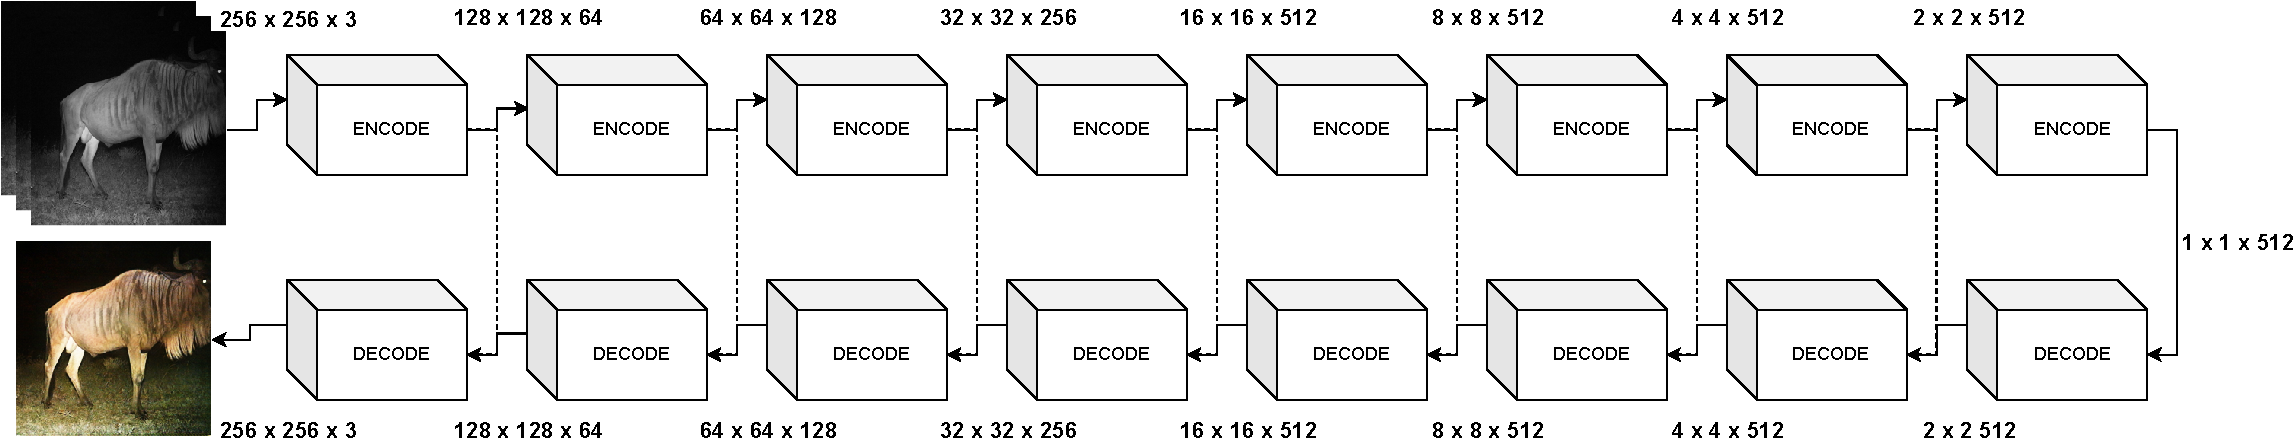
\includegraphics[width=\textwidth]{CycleGAN-Unet.pdf}
   \caption{U-Net generator $G$ used in CycleGAN \cite{unet,mehri2019colorizing}}
   \label{fig:unet}
\end{figure}

\subsubsection*{Optimizations}
Heusel \textit{et al.} demonstrated that using the \textit{two timescale update rule} (TTUR), which states that when the generator and the discriminator have different learning rates,
mode collapse can be prevented in image translation tasks using GANs \cite{ttur}.
Inspired by this, Mehri \textit{et al.} propose utilizing two learning rates for the CycleGAN architecture \cite{mehri2019colorizing}.

Additionally, Mehri \textit{et al.} propose the use of \textit{spectral normalization}, a technique introduced by Miyato \textit{et al.}, to stabilize the training of the discriminators $D_X$ and $D_Y$ \cite{spectral_norm, mehri2019colorizing}.

Finally, Mehri \textit{et al.} observe that while the cycle consistency loss helps in the early training stages, it hinders the network in the later stages in generating realistic images \cite{mehri2019colorizing}.
Therefore, Mehri \textit{et al.} propose to decrease the weight of the cycle consistency loss after half of the training process \cite{mehri2019colorizing}.

\subsection{Contrastive Unpaired Translation (CUT)}
CycleGAN solves the content preservation using a cycle consistency loss which requires duplication of the architecture
of the GAN to have an inverse and also assumes a bijection between the $\mathcal{X}$ and $\mathcal{Y}$ \cite{cyclegan_orig}.
The network is forced to learn a revertible translation, and therefore some freedom for realistic appearance may be lost.
CUT, on the other hand, does not require that the learned function $G$ is invertible.
It encourages content preservation by requiring a patch from the output image e.g., a wildebeest's leg, to be most likely to also come from that patch
of the input image and not from somewhere else in the image, for example the trees in the background \cite{cut}. This is called patchwise contrastive learning (\autoref{fig:cut}).

\begin{figure}[htp!]
   \centering
   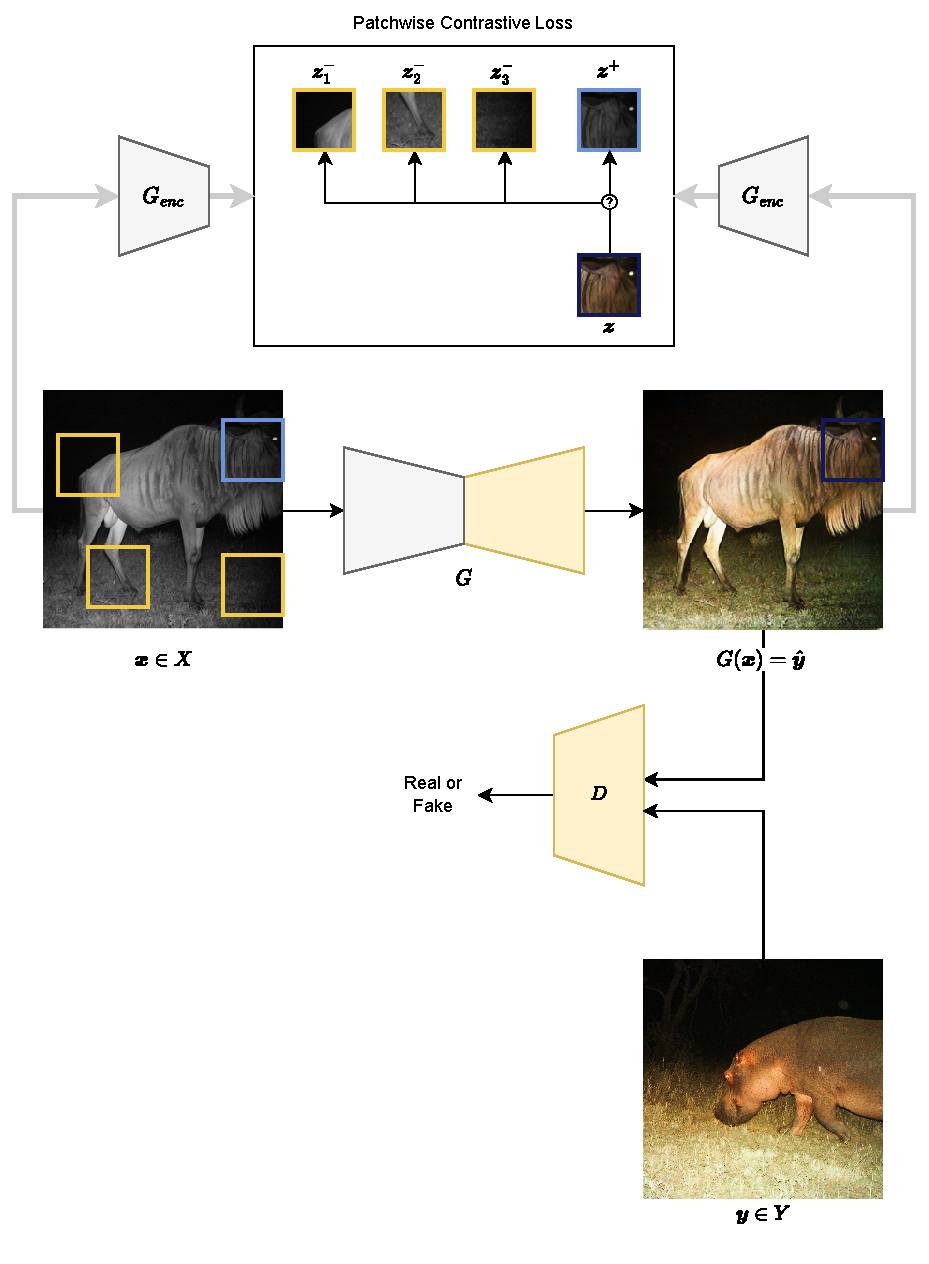
\includegraphics[width=.71\textwidth]{CUT.pdf}
   \caption{
      \textbf{Contrastive Unpaired Translation Schema.}}
   For \textcolor{query}{each query patch} $\ve$ the \textcolor{positive}{corresponding input positive patch} $\vp$ should be associated in contrast to the \textcolor{negative}{negative random input patches} $\vm$.
   The discriminator $D$ encourages the generator to learn the features of domain $\mathcal{Y}$ \cite{cut}.
   \label{fig:cut}
\end{figure}

\subsubsection*{Patch NCE Loss}
First, given a patch of the output image referenced as "query", we want to maximize the probability that the corresponding
patch from the input image, referenced as "positive", would be associated with the query over other input patches referenced
as "negatives" (\autoref{fig:cut}).
The query, the positive, and the $N$ negatives are represented by $K$-dimensional vectors, $\ve \in \mathbb{R}^K$, $\vp \in \mathbb{R}^K$
and $\vm_n \in \mathbb{R}^K$ as the $n$-th negative and $\ve^- \in \mathbb{R}^{N \times K}$.
Subsequently, we can define a cross-entropy loss $l(\ve, \vp, \vm)$ for $\vp$ being associated over $\vm_n$ (\autoref{eqn:patch_loss}).
Note that Park \textit{et al.} added a scaling of $\tau = 0.007$ and normalized the vectors to a unit sphere \cite{cut}.

\begin{equation}
   \label{eqn:patch_loss}
   \begin{aligned}
      l(\ve, \vp, \vm) = - \log \left[ \frac{\exp(\ve \cdot \vp / \tau)}{\exp(\ve \cdot \vp / \tau) + \sum_{i=1}^N\exp(\ve \cdot \ve_n^- / \tau)}\right]
   \end{aligned}
\end{equation}

To obtain those patch representations as $K$-dimensional vectors, Park \textit{et al.} propose to use the already existing
generator function $G$. $G$ is an encoder-decoder network, therefore $G(\x) = G_{dec}(G_{enc}(\x))$, where $G_{enc}$ denotes the encoder \cite{cut}.
Each layer of the encoder network represents multiple patches of the input images. To map this layer to condensed feature vectors,
a small multi-layer perceptron $H_l$ with 2 layers is used, where $H_l$ maps the $l$-th layer of the encoder network to features
$\boldsymbol{z}_l \in \mathbb{R}^{S_l \times C_l}$, therefore $\boldsymbol{z}_l = H_l(G_{enc}^l(\x))$.
$S_l$ is the number of spatial locations and $C_l$ is the size of each feature vector.
For each layer of interest, $l \in \{1, \dots, L\}$ the spatial location $s \in \{1, \dots S_l\}$ inside the layer represents a patch of the input image.
We denote $\boldsymbol{z}_l^s \in \mathbb{R}^{C_l}$ as the feature corresponding to the spatial location, which therefore is a vector representation of a patch
in the input image. All other features of patches in the images are referred to as $\boldsymbol{z}_l^{S \setminus s} \in \mathbb{R}^{(S_l - 1) \times C_l}$.

Now, output query patches are required as features in addition to the features of input image patches. Using the same mechanism on the output image, we can obtain those
$\boldsymbol{\hat{z}}_l = H_l(G_{enc}^l(G(\x)))$. Using the loss defined in \autoref{eqn:patch_loss}, we can obtain a loss for the content preservation of the
GAN $\mathcal{L}_{PatchNCE}(G,H,X)$ \autoref{eqn:patchnce_loss} \cite{cut}.

\begin{equation}
   \label{eqn:patchnce_loss}
   \begin{aligned}
      \mathcal{L}_{PatchNCE}(G,H,X) = \mathbb{E}_{\x \sim X} \sum_{l = 1}^L \sum_{s=1}^{S_l} l(\boldsymbol{\hat{z}}_l^s, \boldsymbol{z}_l^s, \boldsymbol{z}_l^{S \setminus s})
   \end{aligned}
\end{equation}

\subsubsection*{Identity Loss}
Additionally, to the $\mathcal{L}_{PatchNCE}(G, H, X)$ which is applied in the input images, Park \textit{et al.} also proposes to use the loss in the output dataset.
This is a form of identity loss, specific to the domain \cite{cut}.

\subsubsection*{Adversarial Loss}
The adversarial loss as the objective of GAN is an LSGAN loss, therefore $\mathcal{L}_{LSGAN}^G(G, D, X, Y)$ and $\mathcal{L}_{LSGAN}^D(G, D, X, Y)$ are defined
as follows (\autoref{eqn:cut_gan}) \cite{cut}.

\begin{equation}
   \label{eqn:cut_gan}
   \begin{aligned}
      \mathcal{L}_{LSGAN}^D(G, D, X, Y) & = \mathbb{E}_{\y \sim Y}\left[(D(\y) - 0)^2\right] + \mathbb{E}_{\x \sim X}\left[(D(G(\x)) - 1)^2\right] \\
      \mathcal{L}_{LSGAN}^G(G, D, X, Y) & = \mathbb{E}_{\x \sim X}\left[(D(G(\x)) - 0)^2\right]
   \end{aligned}
\end{equation}

\subsubsection*{Full objective}
The final objective $\mathcal{L}$ for the CUT network is defined as follows (\autoref{eqn:cut_total_loss}) \cite{cut}.

\begin{equation}
   \label{eqn:cut_total_loss}
   \begin{aligned}
      \mathcal{L} = \mathcal{L}_{LSGAN}^G(G, D, X, Y) + \mathcal{L}_{PatchNCE}(G,H,X) + \mathcal{L}_{PatchNCE}(G,H,Y)
   \end{aligned}
\end{equation}

\subsubsection*{ResNet}
Contrary to CycleGAN proposed by Mehri \textit{et al.} which uses U-Net \cite{unet} generators \cite{mehri2019colorizing}, CUT uses a generator based on ResNet \cite{cut,resnet}.
While in U-Net the skip connections pass the outputs of encode-blocks to their corresponding decode-blocks, in ResNet, skip connections pass outputs usually a constant amount forward.
A set of layers containing such a skip connection is called \textit{residual block} \cite{resnet}.
The generator used in CUT consists of 9 residual blocks \cite{cut}.

\section{Evaluation}
As NIR colorization has two main application contexts: providing human users more interpretable images and to improve object recognition results by enriching the input with more information.
To assess the effectiveness of both models, we define qualitative evaluation categories and quantitative evaluation metrics based on their ability to achieve these goals.

\subsection{Quantitative Evaluation Metrics}
Due to the unpaired setting, in the quantitative evaluation classic solutions, such as the difference between the absolute intensity values or SSIM \cite{ssim}, cannot be applied. Fortunately, methods for comparing the general image similarity of two sets, such as FID \cite{ttur} or
comparing classification results using an off-the-shelf network, are well known to quantitatively assess the quality of image translation.

\subsubsection*{FID}
To measure how close the generated images are to the real images concerning human perception, the \textit{Fréchet Inception Distance} (FID) \cite{ttur} is a commonly used metric.
It empirically estimates how the human eye perceives images for a set of images and computes the distance between two such set representations.
First, a pre-trained InceptionV3 model evaluates each image of the image set and the activation of the last layer is considered the "human perception approximation".
Then for all activation vectors of the evaluated images in the images set, a multidimensional Gaussian is fitted over those activation vectors.
This is done for two image sets, and later the two Gaussians are compared using the Fréchet distance \cite{ttur}.
Intuitively, if the generated images are realistic, the statistics of features in a classification network should be similar to the real ones.

\subsubsection*{Classification Results}
To satisfy the second application context, that generated images may improve classification results, classification accuracy can be taken into account as a quantitative metric, too.
We generate a train, validation, and test dataset of images generated by the model.
A ResNet-50 \cite{resnet}, with the initial convolutional layer (\texttt{conv1}) frozen, is trained, and the hyperparameters are optimized on the validation dataset.
The network is evaluated on the test dataset, and we use the accuracy as a score for how well the generated images can be handled by recognition systems.
We assume the recognition accuracy to be lower if a network loses content or creates unnatural artifacts.

\subsection{Qualitative Evaluation Methods}
For qualitative evaluation, we define categories on how we determine the superior generated images. These are again based on the two main application contexts.

The first category describes the \textit{naturality} of an image, where the generated images should resemble how humans perceive the world, without artifacts or periodic patterns that can affect visual perception.

The second category refers to the \textit{content preservation} of the input image. This should help humans as well as object detection systems to find and classify animals accurately.

\textit{Hallucinations}, as artifacts or scene elements that are not in the input image, contradict naturality and content preservation, and therefore are undesirable.

\subsection{Network Evaluation For Grayscale Colorization}
\label{sec:suitability-of-cut}

\begin{figure}[ht]
   \centering
   \begin{subfigure}{0.36\textwidth}
      \centering
      \begin{tabular}{l | c}
         Network  & FID $\downarrow$ \\
         \hline \hline
         CycleGAN & 115              \\
         CUT      & \textbf{113}
      \end{tabular}
      \caption{
         \raggedright \textbf{Quantitative Evaluation.} Best FID between grayscale test dataset and RGB images generated by CycleGAN and CUT.
      }
      \label{fig:gray-quan}
   \end{subfigure}
   \hfill
   \begin{subfigure}{0.63\textwidth}
      \centering
      \setkeys{Gin}{width=\linewidth}
      \begin{tabularx}{1\textwidth}{>{\centering\arraybackslash}X >{\centering\arraybackslash}X >{\centering\arraybackslash}X}
         Grayscale \cite{caltech}                                        & CycleGAN                                                             & CUT                                                            \\
         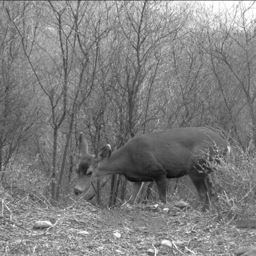
\includegraphics{58ac0e4c-23d2-11e8-a6a3-ec086b02610b_real.png} & 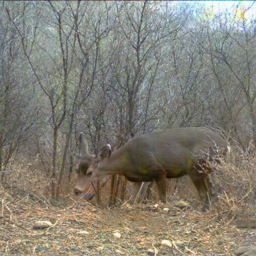
\includegraphics{58ac0e4c-23d2-11e8-a6a3-ec086b02610b_cycle_gan.png} & 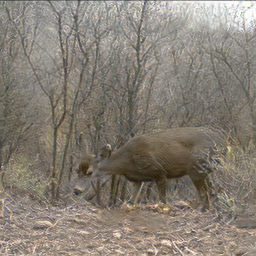
\includegraphics{58ac0e4c-23d2-11e8-a6a3-ec086b02610b_cut.png} \\
         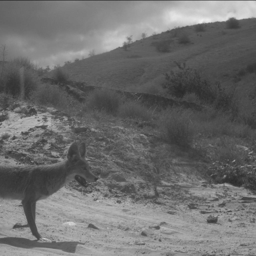
\includegraphics{586e2e43-23d2-11e8-a6a3-ec086b02610b_real.png} & 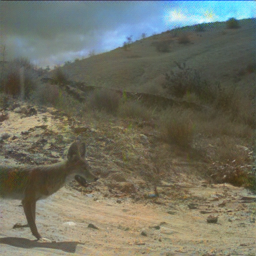
\includegraphics{586e2e43-23d2-11e8-a6a3-ec086b02610b_cycle_gan.png} & 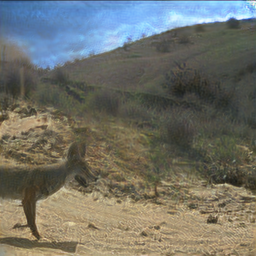
\includegraphics{586e2e43-23d2-11e8-a6a3-ec086b02610b_cut.png} \\
         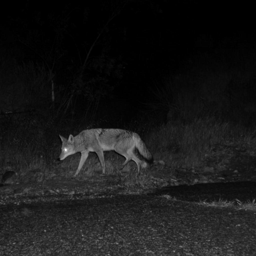
\includegraphics{58782b4f-23d2-11e8-a6a3-ec086b02610b_real.png} & 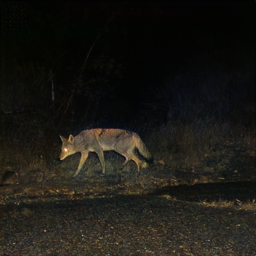
\includegraphics{58782b4f-23d2-11e8-a6a3-ec086b02610b_cycle_gan.png} & 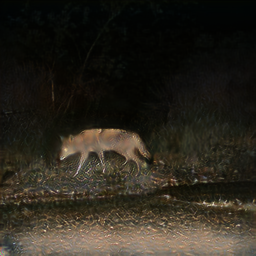
\includegraphics{58782b4f-23d2-11e8-a6a3-ec086b02610b_cut.png}
      \end{tabularx}
      \caption{
         \textbf{Qualitative Evaluation.} Artificial grayscale images with the CCT dataset \cite{caltech} and the corresponding conversion back into the RGB domain by CycleGAN and CUT.
      }
      \label{fig:gray-qual}
   \end{subfigure}
   \caption{
      Evaluation of CycleGAN and CUT trained on an artificial grayscale dataset generated with the CCT dataset \cite{caltech}.
   }
\end{figure}

Both methods are compared in an easier environment.
Different reflection properties of near-infrared light and visual light as well as the unintentional translation between night images (\autoref{sec:time-dependent-sampling}) were excluded while the image colorization remains:
A dataset of unpaired artificial grayscale images (using the mean of all three color channels) and RGB images was created.
We compare the results of CycleGAN and CUT on this dataset.
Although the FID of CUT is slightly better (\autoref{fig:gray-quan}), while it is questionable if such small differences in FID matter, CycleGAN performs slightly better in qualitative evaluation.
In some cases, CUT tends to create artificial textures: The first image has white outlines in the trees, the second image has artificial patterns in the sky (\autoref{fig:gray-qual}) and the third image has such textures on the floor.
In addition to that, CycleGAN and CUT both perform strongly in terms of naturalness and content preservation.

Note that we used $2\cdot10^{-4}$ as the learning rate for CUT training in addition to the hyperparameter suggested \cite{cut}.
For CycleGAN $1.5\cdot10^{-5}$ was used as the generator learning rate and $4.5\cdot10^{-5}$ as the discriminator learning rate where the remaining hyperparameter stay as suggested \cite{mehri2019colorizing}.

\subsection{Network Evaluation For Near Infrared Colorization}
\label{sec:network-comparison}
We evaluate the two architectures CycleGAN and CUT for NIR to RGB transition quantitatively and qualitatively.
A hyperparameter optimization on the validation dataset was done before comparing the resulting networks.
It is noticeable that both networks can create visually appealing and mostly natural-looking images.

While CycleGAN keeps the brightness information from the input image, CUT darkens or brightens animals, especially when they are already near the limit of the illuminated scene.
For example, in the third image of \autoref{fig:network-comparison-qual} the wildebeests in the background are nearly invisible, whereas, in the fourth image, one zebra is too bright (compared to the input image)
and the other zebra is nearly invisible. Therefore, CUT's performance in preserving content is not always satisfactory, in some instances significant details about animals are omitted.

Regarding the FID, a difference of $0.4$ between the networks is not noteworthy (\autoref{fig:network-comparison-quan}).
Based on the classification accuracy results shown in \autoref{fig:network-comparison-quan}, it can be confirmed that CycleGAN outperforms CUT by $9.9\%$.
This provides further evidence on the qualitative observation that CUT tends to lose some information from the input image.

Note that we used $2\cdot10^{-6}$ as the learning rate for CUT training in addition to the suggested hyperparameter \cite{cut}.
For CycleGAN $1.5\cdot10^{-5}$ was used as the generator learning rate and $4.5\cdot10^{-5}$ as the discriminator learning rate where the remaining hyperparameter stay as suggested \cite{mehri2019colorizing}.

\begin{figure}[ht]
   \centering
   \setkeys{Gin}{width=\linewidth}
   \begin{tabularx}{.69\textwidth}{>{\centering\arraybackslash}X >{\centering\arraybackslash}X >{\centering\arraybackslash}X}
      NIR \cite{serengeti}                          & CycleGAN                                          & CUT                                          \\
      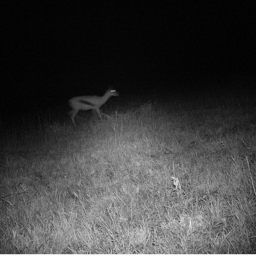
\includegraphics{S2_B07_R1_PICT3274_real.png} & 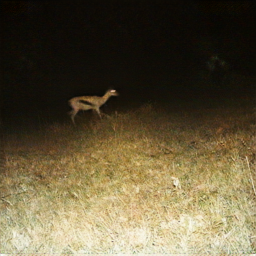
\includegraphics{S2_B07_R1_PICT3274_cyclegan.png} & 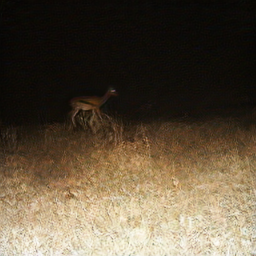
\includegraphics{S2_B07_R1_PICT3274_cut.png} \\
      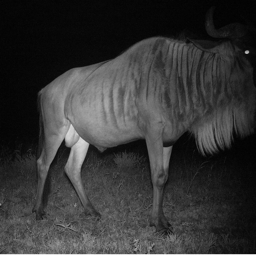
\includegraphics{S2_B07_R3_PICT0492_real.png} & 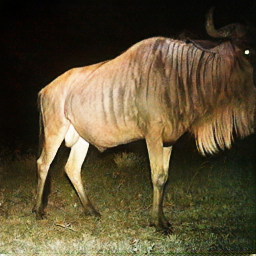
\includegraphics{S2_B07_R3_PICT0492_cyclegan.png} & 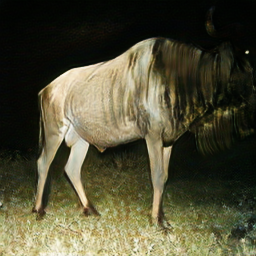
\includegraphics{S2_B07_R3_PICT0492_cut.png} \\
      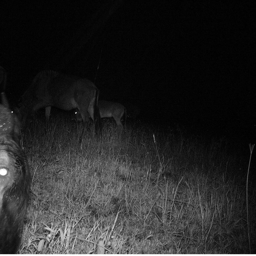
\includegraphics{S2_C07_R1_PICT0675_real.png} & 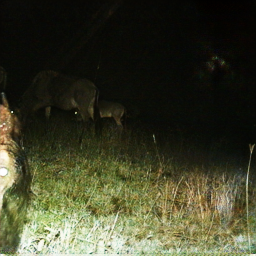
\includegraphics{S2_C07_R1_PICT0675_cyclegan.png} & 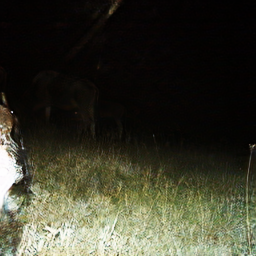
\includegraphics{S2_C07_R1_PICT0675_cut.png} \\
      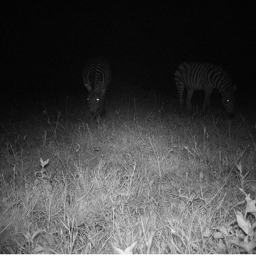
\includegraphics{S2_D08_R1_PICT0080_real.png} & 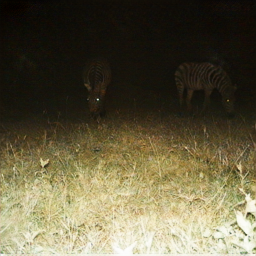
\includegraphics{S2_D08_R1_PICT0080_cyclegan.png} & 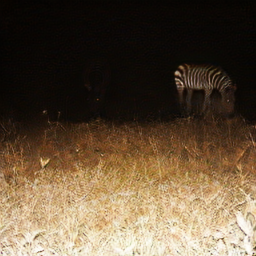
\includegraphics{S2_D08_R1_PICT0080_cut.png} \\
   \end{tabularx}
   \caption{
      \textbf{Qualitative Evaluation.} CycleGAN and CUT trained on Snapshot Serengeti \cite{serengeti} containing only night NIR and RGB images.
      Evaluation on test dataset is done after hyperparameter optimization on validation dataset.
   }
   \label{fig:network-comparison-qual}
\end{figure}


\begin{table}[h]
   \centering
   \begin{tabular}{c | c | c}
      Model    & FID  $\downarrow$ & Classification Accuracy $\uparrow$ \\
      \hline\hline
      CycleGAN & 104.5             & $\mathbf{57.6\%}$                  \\
      CUT      & 104.1             & $52.4\%$
   \end{tabular}
   \caption{
      \textbf{Quantitative Evaluation.} CycleGAN and CUT trained on Snapshot Serengeti \cite{serengeti} containing only night NIR and RGB images.
      Comparing the best FID and classification accuracy obtained on the test dataset.
   }
   \label{fig:network-comparison-quan}
\end{table}

\section{Discussion}
\subsection{Dataset Requirements}
Besides comparing both translation methods, a study on the important points for generating subsets and the suitability of each data source
(CCT and Snapshot Serengeti) as train datasets was performed.

\subsubsection*{Location Dependent Sampling}

\begin{figure}[ht]
   \centering
   \setkeys{Gin}{width=\linewidth}
   \begin{tabularx}{.4\textwidth}{>{\centering\arraybackslash}X >{\centering\arraybackslash}X >{\centering\arraybackslash}X}
      NIR \cite{caltech}                                                  & Generated                                                          \\
      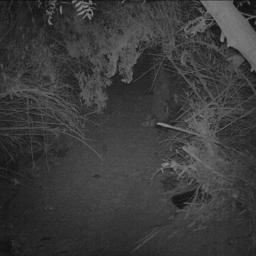
\includegraphics{img/5858c26e-23d2-11e8-a6a3-ec086b02610b_real.png} & 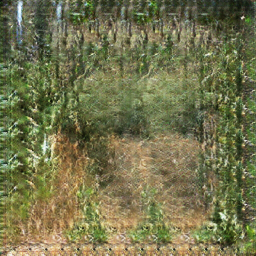
\includegraphics{img/5858c26e-23d2-11e8-a6a3-ec086b02610b_hal.png} \\
      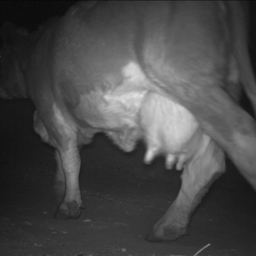
\includegraphics{img/586936d3-23d2-11e8-a6a3-ec086b02610b_real.png} & 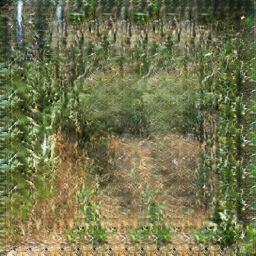
\includegraphics{img/586936d3-23d2-11e8-a6a3-ec086b02610b_hal.png}
   \end{tabularx}
   \caption{
      \textbf{Qualitative Evaluation.} Hallucination \& Mode Collapse because of \textit{dominant location occurrences}.
      CycleGAN was trained on uniform random sampled CCT dataset.
   }
   \label{fig:hallucincation-location}
\end{figure}

Firstly, it proved to be important to not only uniform sample from a dataset to generate a subset, but to take the location occurrence into account.
The occurrence of certain locations is frequent in both datasets and, as a result, they can significantly influence the training.
Mode collapse, such that specific features of a location are generated independently of whether they are in the input image or not, are
observable results (\autoref{fig:hallucincation-location}). A weighted sampling based on the location and random cropping of images can solve this problem.

\subsubsection*{Time Dependent Sampling}
\label{sec:time-dependent-sampling}

\begin{figure}[ht]
   \centering
   \begin{subfigure}{0.34\textwidth}
      \centering
      \begin{tabular}{l | c}
         Train Dataset & FID $\downarrow$ \\
         \hline \hline
         Random        & 203.15           \\
         Only Night    & 149.51
      \end{tabular}
      \caption{
         \raggedright \textbf{Quantitative Evaluation.} Best FID between RGB CCT test dataset and generated RGB using CCT NIR test dataset as input for each network (Random, Only Night)
      }
      \label{fig:hallucation-night-day-quan}
   \end{subfigure}
   \hfill
   \begin{subfigure}{0.65\textwidth}
      \centering
      \setkeys{Gin}{width=\linewidth}
      \begin{tabularx}{\textwidth}{>{\centering\arraybackslash}X >{\centering\arraybackslash}X >{\centering\arraybackslash}X}
         NIR  \cite{caltech}                                             & Random                                                         & Only Night                                                             \\
         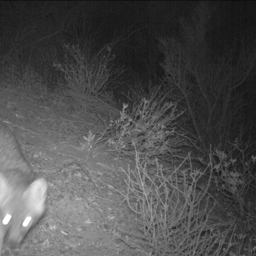
\includegraphics{586ae0f6-23d2-11e8-a6a3-ec086b02610b_real.png} & 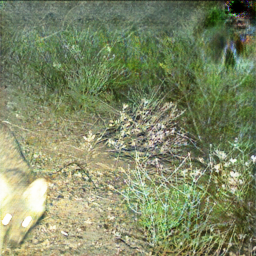
\includegraphics{586ae0f6-23d2-11e8-a6a3-ec086b02610b_hal.png} & 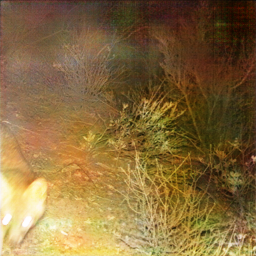
\includegraphics{586ae0f6-23d2-11e8-a6a3-ec086b02610b_without_hal.png} \\
         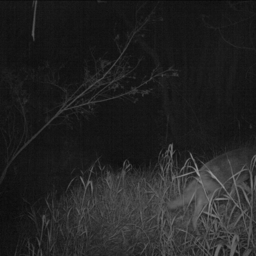
\includegraphics{588c13ba-23d2-11e8-a6a3-ec086b02610b_real.png} & 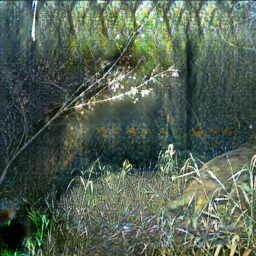
\includegraphics{588c13ba-23d2-11e8-a6a3-ec086b02610b_hal.png} & 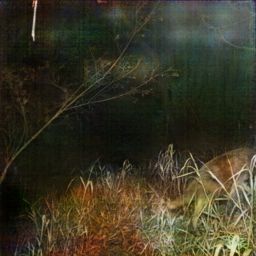
\includegraphics{588c13ba-23d2-11e8-a6a3-ec086b02610b_without_hal.png}
      \end{tabularx}
      \caption{
         \textbf{Qualitative Evaluation.} Evaluation of the two networks Random, Only Night on the CCT test dataset NIR images \cite{caltech}.
      }
      \label{fig:hallucation-night-day-qual}
   \end{subfigure}
   \caption{
      Hallucination because of \textit{unintended night-to-day translation}: 
      Comparison of two training datasets used to train CycleGAN. Random is CycleGAN trained on time independent sampled dataset of NIR images.
      Only Night is CycleGAN trained on only night NIR and RGB images (using Snapshot Serengeti dataset \cite{serengeti}).
   }
   \label{fig:hallucincation-night-day}
\end{figure}

Secondly, just providing random NIR and RGB for training also proved to be not optimal.
Commonly, camera traps take NIR images at night and RGB images during the day.
Therefore, when random NIR and RGB images are sampled, the near-infrared images are mostly from the night and the RGB images from the day.
This leads to the discriminator anticipating real RGB images to have daylight features such that the far points in the image are still visible and that the sky should be visible and preferably blue/gray.
Consequently, the generator tries to satisfy the discriminator and invents those features while translating.
Because night images do not have the information for those features, the network invents them.
This effect is called \textit{hallucination}. It results in a substantial FID increase (\autoref{fig:hallucation-night-day-quan}) and invention of information, as
well as artifacts in the output image (\autoref{fig:hallucation-night-day-qual}).
This problem can be solved by using only night images for training (\textbf{Only Night} in \autoref{fig:hallucation-night-day-qual}).

Using the given timestamps on the COCO metadata of the CCT dataset \cite{caltech} a sampling of only night images failed due to too less RGB night images.
Snapshot Serengeti, on the other hand, used two types of cameras during the survey:
Scoutgard's SG565 cameras which produce RGB \textbf{night} images using an \textit{incandescent} flash and
DLC Covert II cameras which use an infrared flash, and therefore produce NIR night images \cite{serengeti}.
Thus, the Snapshot Serengeti Dataset is preferable to the CCT dataset as a training dataset for NIR to RGB night translation.

\subsection{Network Comparison}
The final results show that both networks perform strongly on qualitative and quantitative evaluation (\autoref{fig:network-comparison-quan} and \autoref{fig:network-comparison-qual}). Overall, CycleGAN performs slightly better.

Park \textit{et al.} could create substantially better results with a contrastive loss instead of cycle consistency loss in their experiments \cite{cut}.
Park \textit{et al.} used the original CycleGAN for comparison \cite{cut} while we use a CycleGAN which is specifically tuned for NIR colorization \cite{mehri2019colorizing}.
This can at least partially explain the difference.
In addition, it was \textit{hypothesized} that due to the contrastive loss of CUT, which attempts to assign patches from the output image to the corresponding patch from the input image
\textit{in contrast} to other patches from the input image, CUT cannot show significant improvements compared to CycleGAN when applied to whole images.
Intuitively, it might be easier to assign such distinct parts as a horse head to a zebra head compared to assigning a colored scrub in the background exactly its corresponding NIR patch.
Those images with regions that lack distinct features which must be transformed (like NIR $\rightarrow$ RGB translation) may not benefit greatly from the usage of CUT.
On the other hand, CUT can show large performance improvements compared to CycleGAN in partial image translation, such as translating horses into zebras, as Park \textit{et al.} did \cite{cut}.

\begin{table}[ht]
   \centering
   \begin{adjustbox}{width=1\textwidth}
      \begin{tabular}{l | >{\centering\arraybackslash} p{5.5cm} | >{\centering\arraybackslash} p{3cm} | >{\centering\arraybackslash} p{3.5cm} }
         Model                                                               &
         Cityscapes (Semantic $\rightarrow$ Image) \newline FID $\downarrow$ &
         Horse $\rightarrow$ Zebra \newline FID $\downarrow$                 &
         Winter $\rightarrow$ Summer \newline FID $\downarrow$                                       \\
         \hline\hline
         CycleGAN \cite{cyclegan_orig}                                       & 75.97 & 76.37 & 86.14 \\
         CUT \cite{cut}                                                      & 57.16 & 45.33 & 80.25
      \end{tabular}
   \end{adjustbox}
   \caption{
      \textbf{Quantitative Comparison.} (FID) of CUT and CycleGAN for multiple datasets \cite{monce}.
      Horse $\rightarrow$ Zebra: images of horses to zebras without changing the environment or posture of the animal (partial image translation).
      Cityscape (Semantic $\rightarrow$ Image): semantic images of streets to streets (whole image translation with some distinct features).
      Winter $\rightarrow$ Summer: landscapes in winter translated to summer (whole image translation with less distinct features).
   }
   \label{fig:cut-cycle-gan-datasets-quan}
\end{table}

Zhan \textit{et al.} compared CycleGAN and CUT as their baseline models. Although CUT drastically improved quantitative results for the Horse $\rightarrow$ Zebra dataset ($\sim68\%$ improvement) or for the Cityscapes dataset
($\sim 35\%$ improvement), the improvement for the Winter $\rightarrow$ Summer dataset was quite small ($\sim 7\%$ improvement) (\autoref{fig:cut-cycle-gan-datasets-quan})\cite{monce}.
Since the Winter $\rightarrow$ Summer dataset has in contrast to Horse $\rightarrow$ Zebra and Cityscapes only a few distinct features and translates the whole image, it may be similar to the NIR $\rightarrow$ RGB scenario.
This indicates that the improvement of CUT compared to CycleGAN in the NIR $\rightarrow$ RGB could also be small.

We test our hypothesis by abstracting away difficult parts of the NIR to RGB translation, which are the different reflection properties of visual and near-infrared light as well as the unwanted suggestion to translate from night to day.
The property of translating a whole image with many regions that lack distinct features (like the background in those images), but must also be translated, remains.
As shown in \autoref{sec:suitability-of-cut} CUT does not show notable performance improvements to our improved version of CycleGAN.
This provides support for this hypothesis, although it should be tested more thoroughly.
Independently, this indicates that the similarities in performance between CUT and CycleGAN are observable not only for the more difficult NIR image colorization, but also for the much simpler grayscale image colorization.

For CUT, a lower accuracy than for CycleGAN could be observed in \autoref{sec:network-comparison} (\autoref{fig:network-comparison-quan}).
In addition, qualitatively an information loss was also noticeable \autoref{fig:network-comparison-qual}.
Since CUT does not require the generator to produce a revertible transformation, it is not obliged to preserve the content as strictly (\autoref{fig:cut}).
The noticed effect may be traced back to this design element of the architecture.

Furthermore, Park \textit{et al.} noted that CUT trains faster than the original CycleGAN.
For this improved version of CycleGAN, this does not hold anymore.
In particular, U-Net generators drastically improve computational time.
Additionally, CUT is usually trained with $400$ epochs, while CycleGAN only trains $200$ for epochs to achieve similar results.
This results in much more computational time needed to train CUT ($\sim 30$ hours) compared to CycleGAN ($\sim$ 13 hours).

\section{Conclusion}
We showed that both methods, CycleGAN using a cycle consistency loss \cite{mehri2019colorizing} and CUT using a contrastive loss \cite{cut}, can learn a translation function between the NIR- and RGB domain that produces natural-looking images.
This provides tools for wildlife researchers to enhance their understanding and interpretation of the visual data obtained from NIR images.
Creating a dataset of both near-infrared and incandescent images showed to play a major role in the success of the translation.
Therefore, a dataset providing near-infrared and incandescent images as Snapshot Serengeti \cite{serengeti} should be used.
CUT did not show significant improvements compared to CycleGAN, as expected \cite{cut}.
This also holds for the simpler case of grayscale colorization.
We hypothesize reasons for that, but further investigations on which problems CUT is best suited may be a future field of research.
Since we used CUT in the original version, tuning CUT for NIR colorization, e.g., using U-Net \cite{unet}, relativistic GAN losses \cite{rel_gan}, TTUR \cite{ttur} or other optimizations
could improve the performance of CUT in NIR colorization and therefore would make it superior to CycleGAN.

Moreover, we only briefly addressed the potential of utilizing colorization to improve the classification.
Other lighter network architectures could be tested to first see if there can be a positive impact on the classification compared to using colorized NIR images.
Alternatively, an ensemble network using a network for classifying NIR images and a network for classifying colorized NIR images as done by Gao \text{et al.} \cite{cyclegan_camera_traps} could increase the performance.
Confidence normalization \cite{guo2017calibration} could be used to choose which classification result should be used.

\printbibliography

\end{document}